\chapter{时序图查询模块的设计与实现}
时序RDF图和时序超图查询系统是受关注相对较少的研究方向,即使已经出现了一些面向时序RDF图的图查询系统,但它们的性能较差,查询响应时间和并发处理能力都难以令人满意,时序超图查询系统的研究更是少有人问津。本章将介绍\sys 的时序图查询模块,它在Wukong的基础上对时序图查询进行了针对性的优化,实现了时序RDF图和时序超图的可扩展存储和高效查询。

\section{时序图查询语言}
RDF的标准查询语言SPARQL并没有与时序相关的语法,所以需要在SPARQL原有语法的基础上进行时序扩展,以支持时序数据的查询。超图并没有其标准的查询语言,时序超图当然也没有,所以我们同样需要设计时序超图的查询语言。

\subsection{时序RDF图查询语言SPARQL-T}
本文设计的时序RDF图查询语言SPARQL-T从两方面对SPARQL的语法进行了扩展:
\begin{itemize}
\item 将GP中的“主语-谓词-宾语”三元模式扩展为“主语-谓词-宾语-有效时间区间的开始时间-有效时间区间的截止时间”五元模式(QP),新加入的两个元素要求是变量,用来获取时序三元组的有效时间数据。为了兼容标准的SPARQL语法,我们规定新加入的两个元素是可选的,但它们要么同时存在,要么同时不存在。
\item GP中的过滤器可以对时间变量的取值按照一定条件进行过滤,例如与变量或常量的大小关系比较等。
\end{itemize}

\begin{figure}[!htb]
\center{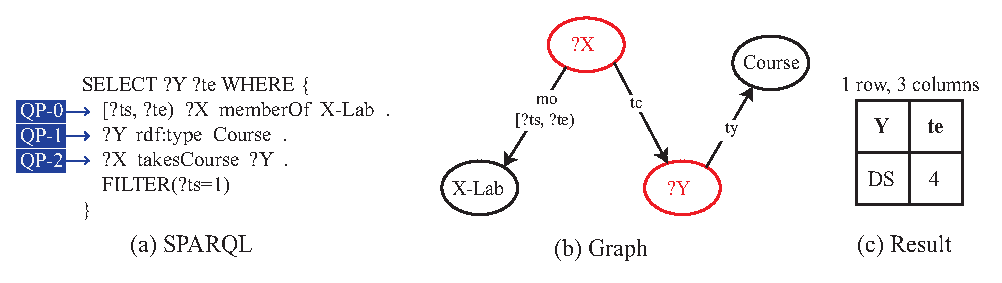
\includegraphics[width=0.9\textwidth]  {figures/tsparql.eps}} 
\bicaption{示例时序RDF图上的一条SPARQL-T查询语句}{A SPARQL-T query statement on the temporal RDF graph example}
\label{tsparql}
\end{figure}

图\ref{tsparql}给出了一条图\ref{trdf}中的时序RDF图上的SPARQL-T语句示例。
QP-0包含两个时间变量\texttt{ts}和\texttt{te},它们应该分别取值为匹配到的时序三元组的有效时间区间的开始时间和截止时间。
GP还包含一个过滤器,它会过滤出变量\texttt{ts}的取值为1的查询结果条目。
GP中的三个模式构成了图\ref{tsparql}(b)所示的查询图,可以在图\ref{trdf}中的时序RDF图上找到一个与之匹配的子图,
过滤后得到的查询结果如图\ref{tsparql}(c)所示,共一行二列。

\subsection{时序超图查询语言HQL-T}
时序超图是一种表示集合关系的数据模型,所以时序超图查询语言应该着重查询\textbf{集合间的关系}(即时序超边间的关系)、\textbf{元素和集合间的关系}(即顶点和时序超边间的关系)以及\textbf{元素间的关系}(即顶点间的关系)。此外,时序超图查询语言也应当支持\textbf{对时序超边的有效时间的查询}以及\textbf{基于有效时间的筛选}。

HQL-T查询语句的基础形式依然是
\begin{equation}
    \mathtt{SELECT \ RD \ WHERE \ GP}
\end{equation}
其中GP由一组基础关系模式(RP)组成,也可以包含过滤器,过滤器和RD的作用与SPARQL-T中的相同。给定一个时序超图$G$和一个HQL-T查询语句$Q$,HQL-T执行引擎会根据GP指定的模式在$G$中搜索与之匹配的子结构,找到RD中所有变量的可取值。RP的基本结构为:
\begin{equation}
    \mathtt{input \ builtin\colon \! type(args) \ output \ interval}
\end{equation}
其中\texttt{input}是输入元素列表,\texttt{builtin}是内置关键字,\texttt{type}指定了该模式的类型,\texttt{args}是该模式的参数,\texttt{output}是输出元素列表。\texttt{interval}是可选的,它是一个由两个变量组成的区间,格式为\texttt{[?var$_1$,?var$_2$)},当它出现在RP中时,HQL-T执行引擎应当将变量\texttt{var$_1$}和\texttt{var$_2$}分别取值为使得此RP成立的时间区间的开始时间和截止时间。
根据\texttt{type}的值,RP可分为以下几类:

\begin{figure}[!htb]
\center{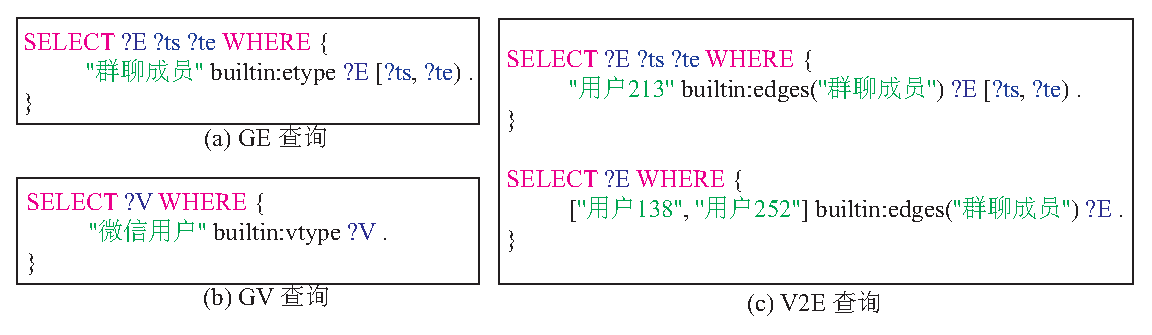
\includegraphics[width=0.9\textwidth]  {figures/hqls1.eps}} 
\bicaption{HQL-T查询语句示例(1)}{HQL-T query statement example (1)}
\label{hql1}
\end{figure}

\begin{itemize}
\item \textbf{GE模式:}该类型RP的\texttt{type}为\texttt{etype},输入元素列表要求只包含一个表示时序超边类型的常量;输出元素列表要求只包含一个变量;没有参数。这类RP的作用是查询所有指定类型的时序超边。如果包含\texttt{interval},那么变量\texttt{var$_1$}和\texttt{var$_2$}会分别取值为查询到的时序超边的有效时间区间的开始时间和截止时间。图\ref{hql1}(a)给出了一条只包含GE模式的HQL-T查询语句示例,该查询是要查找所有类型为“群聊成员”的时序超边。
\item \textbf{GV模式:}该类型RP的\texttt{type}为\texttt{vtype},输入元素列表要求只包含一个表示顶点类型的常量;输出元素列表要求只包含一个变量;没有参数。这类RP的作用是查询所有指定类型的顶点。由于顶点没有时序数据,所以\texttt{interval}不能出现在这类RP中。图\ref{hql1}(b)给出了一条只包含GV模式的HQL-T查询语句示例,该查询是要查找所有类型为“微信用户”的顶点。
\item \textbf{V2E模式:}该类型RP的\texttt{type}为\texttt{edges},输入元素列表可以包含若干表示顶点的常量或变量,输出元素列表要求只包含一个表示时序超边的变量,参数必须是一个表示时序超边类型的常量。这类RP的作用是查找所有指定类型且同时包含各输入顶点的时序超边。如果包含\texttt{interval},那么变量\texttt{var$_1$}和\texttt{var$_2$}会分别取值为查询到的时序超边的有效时间区间的开始时间和截止时间。图\ref{hql1}(c)给出了两条只包含V2E模式的HQL-T查询语句示例,第一个查询是要查找所有类型为“群聊成员”且包含顶点“用户213”的时序超边,第二个查询是要查找所有类型为“群聊成员”且同时包含顶点“用户138”和“用户252”的时序超边。
\end{itemize}

\begin{figure}[!htb]
\center{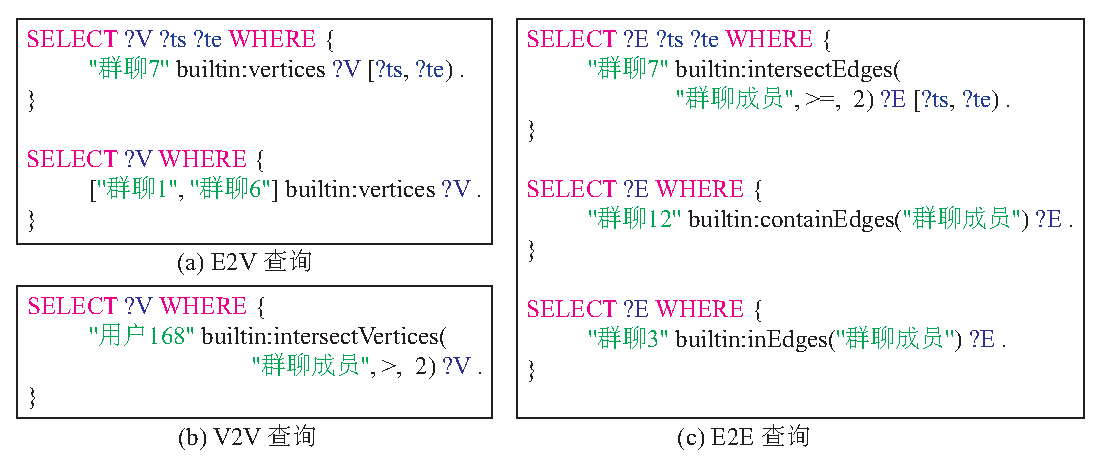
\includegraphics[width=0.9\textwidth]  {figures/hqls2.eps}} 
\bicaption{HQL-T查询语句示例(2)}{HQL-T query statement example (2)}
\label{hql2}
\end{figure}

\begin{itemize}
\item \textbf{E2V模式:}该类型RP的\texttt{type}为\texttt{vertices},输入元素列表可以包含若干表示时序超边的常量或变量,输出元素要求只包含一个表示顶点的变量,没有参数。这类RP的作用是查找各输入时序超边包含的所有公共顶点。如果包含\texttt{interval},那么变量\texttt{var$_1$}和\texttt{var$_2$}会分别取值为能够使得各输入时序超边都有效的最大时间区间的开始时间和截止时间。图\ref{hql2}(a)给出了两条只包含E2V模式的HQL-T查询语句示例,第一个查询是要查找时序超边“群聊7”的有效时间区间和包含的所有顶点,第二个查询是要查找时序超边“群聊1”和“群聊6”包含的公共顶点。
\item \textbf{V2V模式:}该类型RP的\texttt{type}为\texttt{intersectVertices},输入元素列表可以包含若干表示顶点的常量或变量,输出元素要求只包含一个表示顶点的变量。要求有三个参数,第一个参数是时序超边的类型,第二个参数是比较运算符,可以是$>$、$<$、$=$、$!=$、$>=$和$<=$其中之一,该参数可以省略,省略时默认是$>=$,第三个参数是一个整数。这类RP的作用是查找同时与各输入顶点出现在相同时序超边的顶点,且时序超边的类型和数量要满足参数的要求。这类RP不能包含\texttt{interval}。图\ref{hql2}(b)给出了一条只包含V2V模式的HQL-T查询语句示例,该查询是要查找与顶点“用户168”同时加入超过2个共同群聊的顶点。
\item \textbf{E2E模式:}该类型RP的\texttt{type}为\texttt{intersectEdges}、\texttt{containEdges}或\texttt{inEdges},输入元素列表可以包含若干表示时序超边的常量或变量,输出元素要求只包含一个表示时序超边的变量。当\texttt{type}为\texttt{intersectEdges}时,要求有三个参数,第一个参数是时序超边的类型,第二个参数是比较运算符,可以是$>$、$<$、$=$、$!=$、$>=$和$<=$其中之一,该参数可以省略,省略时默认是$>=$,第三个参数是一个整数,这类RP的作用是查找与各输入时序超边的交集的基数满足参数要求的时序超边;当\texttt{type}为\texttt{containEdges}或\texttt{inEdges}时,参数必须是一个表示时序超边类型的常量,这类RP的作用是查找指定类型且是各输入时序超边子集(当\texttt{type}为\texttt{containEdges}时)或超集(当\texttt{type}为\texttt{inEdges}时)的时序超边。如果包含\texttt{interval},那么变量\texttt{var$_1$}和\texttt{var$_2$}会分别
取值为能够使得各输入、输出时序超边同时有效的最大时间区间的开始时间和截止时间。图\ref{hql2}(c)给出了三个只包含E2E模式的HQL-T查询语句示例,第一个查询是要查找与时序超边“群聊7”拥有不少于2个公共顶点的类型为“群聊成员”的时序超边,第二个查询是要查找所有顶点都在时序超边“群聊12”中且类型为“群聊成员”的时序超边,第三个查询是要查找包含时序超边“群聊3”的所有顶点且类型为“群聊成员”的时序超边。
\end{itemize}

以上六类RP的组合可以实现很强的查询语义,基本可以满足对时序超图的查询需求。对于包含多RP的HQL-T查询语句,查询引擎需要按序逐条执行各RP。图\ref{hql}是一条包含两个RP的查询语句,在执行该语句时,需要先找到所有类型为“群聊成员”的时序超边,然后将找到的所有时序超边依次作为输入元素,查找其包含的所有顶点,最后过滤出符合条件的查询结果。

\begin{figure}[!htb]
\center{
\includegraphics[width=0.8\textwidth]  {figures/hql.eps}}
\bicaption{普通HQL-T查询语句示例}{Common HQL-T query statement example}
\label{hql}
\end{figure}
\section{时序RDF图存储结构和查询引擎}
时序RDF图的存储主要是基于\S\ref{chap:kvstore}中介绍的分布式键值存储实现的,在此基础上,它还使用分布式排序数组结构加速时间条件查询。时序RDF图查询引擎使用存储层提供的接口、按照用户指定的查询计划执行SPARQL-T查询语句中GP的各模式。本节将详细介绍时序RDF图的存储结构和查询引擎。
\subsection{存储结构}
\label{sec:rdfstore}
如\S\ref{sec:arch}所述,\sys 并不直接存储时序RDF图数据集中的字符串,而是将其转化成整型ID进行存储,并使用字符串服务器管理字符串和整型ID之间的对应关系。时序RDF图数据集中的字符串分为两类:
\begin{enumerate}
\item 时序三元组中表示谓词的字符串及表示类型名的字符串,例如时序三元组\texttt{Eric memberOf X-Lab [1,2)}中的\texttt{memberOf}和时序三元组\texttt{Eric rdf:type Student [0,+$\infty$)}中的\texttt{rdf:type}、\texttt{Student}。
这类字符串对应的ID范围为$[1,2^{17})$,特别地,\texttt{rdf:type}对应的ID为1。
本文将表示谓词的字符串对应的ID称为\texttt{pid},将表示类型名的字符串对应的ID称为\texttt{tid}。
\item 时序三元组中表示主语和宾语的字符串(表示类型名的字符串除外),例如时序三元组\texttt{Eric memberOf X-Lab [1,2)}中的\texttt{Eric}和\texttt{X-Lab}。这类字符串对应的ID范围为$[2^{17},2^{46})$。本文将这类字符串对应的ID称为\texttt{vid}。
\end{enumerate}

系统默认使用32位UINT表示各种ID,对于规模比较庞大的数据集,可以在系统编译时指定使用64位UINT。

时序RDF图存储内存布局如图\ref{trdfstore},分为键值存储区和时序三元组存储区两部分。
时序三元组存储区本质上是内存数组,它分为两部分,在“时序三元组存储1”中,时序三元组按照有效时间区间的开始时间升序排布;在“时序三元组存储2”中,时序三元组按照有效时间区间的截止时间升序排布。
键值存储区中的键值对分为直接索引和间接索引两类,在直接索引中,值是实际数据;在间接索引中,值由指向“时序三元组存储1”中时序三元组的指针组成。

\begin{figure}[!htb]
\center{
\includegraphics[width=0.6\textwidth]  {figures/trdfstore.eps}}
\bicaption{时序RDF图存储内存布局}{Temporal RDF graph storage memory layout}
\label{trdfstore}
\end{figure}

在键值存储区中,各种键值对及其类型如表\ref{tab:trdf}所示。键的数据类型是64位UINT,由三部分组成,第一部分使用其高46位,第二部分使用其中间17位,第三部分使用其最低位。第三部分只能是OUT(1,表示出方向)和IN(0,表示入方向)其中之一。值的基本数据类型与ID的数据类型相同,可以是32或64位UINT,这取决于系统编译时的配置。
\begin{table}[!hpt]
  \bicaption{时序RDF图存储使用的键值对}{Key-value pairs used in temporal RDF graph storage}
  \label{tab:trdf}
  \centering
  \begin{tabular}{p{1cm}p{3cm}p{8cm}p{2cm}} \toprule
    序号 & 键 & 值 & 类型 \\ \midrule
    1\centering & \texttt{[0|0|OUT]} & 所有\texttt{pid} & \multirow{8}{*}{直接索引} \\
    2\centering & \texttt{[0|1|OUT]} & 所有\texttt{tid} & \\
    3\centering & \texttt{[0|1|IN]} & 所有\texttt{vid} & \\
    4\centering & \texttt{[0|tid|IN]} & 所有类型为\texttt{tid}的\texttt{vid} & \\
    5\centering & \texttt{[0|pid|OUT]} & 谓词为\texttt{pid}的所有时序三元组中所有表示宾语的\texttt{vid} & \\
    6\centering & \texttt{[0|pid|IN]} & 谓词为\texttt{pid}的所有时序三元组中所有表示主语的\texttt{vid} & \\
    7\centering & \texttt{[vid|0|OUT]} & 主语为\texttt{vid}的所有时序三元组中的所有\texttt{pid} & \\
    8\centering & \texttt{[vid|0|IN]} & 宾语为\texttt{vid}的所有时序三元组中的所有\texttt{pid} & \\ 
    \hline
    9\centering & \texttt{[vid|1|OUT]} & 描述\texttt{vid}类型的时序三元组 & \multirow{3}{*}{间接索引} \\ 
    10\centering & \texttt{[vid|pid|OUT]} & 主语为\texttt{vid}、谓词为\texttt{pid}的所有时序三元组 & \\ 
    11\centering & \texttt{[vid|pid|IN]} & 宾语为\texttt{vid}、谓词为\texttt{pid}的所有时序三元组 & \\ 
    \bottomrule
  \end{tabular}
\end{table}

图\ref{trsdemo}给出了系统会为图\ref{trdf}中的数据集生成的一部分键值对。为了便于理解,图中使用字符串表示主语、谓词和宾语,系统实际使用的是这些字符串对应的ID。
在间接索引中,值是一个由时序三元组在“时序三元组存储1”中的偏移量组成的列表,例如,时序三元组\texttt{Kurt memberOf X-Lab [1,4)}在“时序三元组存储1”中的偏移量为5,那么间接索引就使用5来表示该时序三元组。

\begin{figure}[!htb]
\center{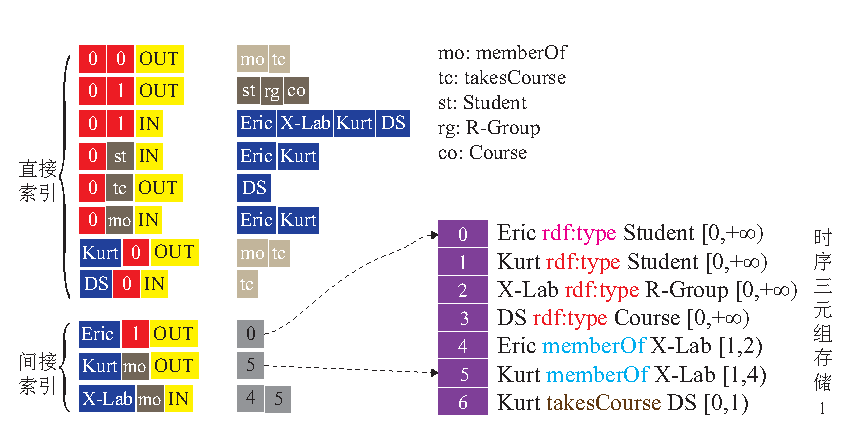
\includegraphics[width=0.75\textwidth]  {figures/trsdemo.eps}}
\bicaption{时序RDF图存储使用的键值对示例}{Example of key-value pairs used in temporal RDF graph storage}
\label{trsdemo}
\end{figure}

为了实现RDF数据集的分布式可扩展存储,系统使用如下规则将键值对和时序三元组划分到各查询节点中存储:
\begin{enumerate}
    \item 每个查询节点负责一部分\texttt{vid}的管理,\texttt{vid}会被分配到的查询节点(查询节点从0开始编号)为:
    \begin{equation}
        \mathtt{vid \ \% \ num\_qnodes}
    \end{equation}
    其中\texttt{num\_qnodes}是查询节点数。
    \item 对于键值对1-6,将值按照1中的规则划分到各查询节点存储,同一键会出现在每个查询节点的键值存储中;对于键值对7-11,将键依据其第一部分按照1中的规则划分到不同查询节点存储,每个键只会出现在一个查询节点的键值存储中。
    \item 将所有时序三元组分别按有效时间区间的开始时间和截止时间排序后,分别按块划分到各查询节点的“时序三元组存储1”和“时序三元组存储2”中存储,偏移量为\texttt{off}的时序三元组会被分配到的查询节点(从0开始编号)为:
    \begin{equation}
        \mathtt{off \ / \ \lceil num\_ttriples \ / \ num\_qnodes \rceil}
    \end{equation}
    其中\texttt{num\_ttriples}是时序三元组总数。
\end{enumerate}

分布式键值存储结构可以实现高效的拓扑查询,两个“时序三元组存储”可以实现高效的时间条件查询。对于以时序三元组有效时间区间开始时间为条件的查询,可以在“时序三元组存储1”上通过二分法快速找到目标时序三元组,同理可以使用“时序三元组存储2”快速处理以时序三元组有效时间区间截止时间为条件的查询。直接索引和间接索引相结合的键值存储结构可以在实现高效的拓扑查询和时间条件查询的同时,减少时序数据存储占用的空间。

表\ref{tab:storeif}列出了存储层向上提供的接口,接口\ding{182}只涉及对本节点上键值存储结构的读,接口\ding{183}可能涉及对各节点的键值存储结构和“时序三元组存储1”的读,接口\ding{184}和\ding{185}可以分别筛选出本节点的“时序三元组存储1”和“时序三元组存储2”中符合时间条件的时序三元组。
\begin{table}[!hpt]
  \bicaption{时序RDF图存储提供的接口}{Interfaces provided by temporal RDF graph storage}
  \label{tab:storeif}
  \centering
  \begin{tabular}{p{1cm}p{8cm}p{5.5cm}} \toprule
    序号 & 接口 & 作用 \\ \midrule
    \ding{182}\centering & \texttt{list<value\_t> get\_values(key)} & 获取本节点上键\texttt{key}对应的值列表,适用于键值对1-6 \\
    \ding{183}\centering & \texttt{list<triple\_t> get\_ttriples(key)} & 获取键\texttt{key}对应的时序三元组列表,适用于键值对7-11 \\
    \hline
    \ding{184}\centering & \texttt{list<triple\_t> get\_ttriples\_ts(start, end)} & 从本节点的“时序三元组存储1”中获取所有有效时间区间开始时间范围为\texttt{[start,end]}的时序三元组 \\
    \ding{185}\centering & \texttt{list<triple\_t> get\_ttriples\_te(start, end)} & 从本节点的“时序三元组存储2”中获取所有有效时间区间截止时间范围为\texttt{[start,end]}的时序三元组 \\
    \bottomrule
  \end{tabular}
\end{table}

\subsection{查询引擎}
SPARQL-T查询引擎沿用了Wukong使用的图探索和全历史剪枝算法。
默认情况下,查询引擎会使用存储层提供的接口\ding{182}和\ding{183}通过键值存储查找所需的数据,但对于一些以时间点或时间范围为条件的查询,通过接口\ding{184}和\ding{185}直接从“时序三元组存储”中寻找符合条件的时序三元组可能更加高效。
例如图\ref{tsparql}中的查询语句想要找到满足如下条件的资源Y:Y的类型是课程且有加入X-Lab时间为1的X-Lab成员选修该课程。
在执行该语句时,可以先在“时序三元组存储1”中快速找到有效时间区间开始时间为1的时序三元组,然后再对这些时序三元组做进一步筛选。如果查询引擎不直接使用“时序三元组存储”,而是先使用键值存储做图探索,然后再筛选出变量\texttt{ts}的取值为1的查询结果,那么就会带来更大的数据访问开销。用户可以通过在GP中使用\textbf{时序三元组时间范围模式}显式地要求查询引擎使用“时序三元组存储”进行时间条件查询,语法为:
\begin{equation}
    \mathtt{interval \ s \ p \ o \ STRAT/END(const_1, const_2)}
\end{equation}
其中\texttt{s}、\texttt{p}和\texttt{o}分别表示时序三元组的主语、谓词和宾语,它们都可以是常量或变量;\texttt{interval}是可选的,它是一个由两个变量组成的区间,格式为\texttt{[?var$_1$,?var$_2$)},当它存在时,两个变量会分别取值为查询到的时序三元组的有效时间区间的开始时间和截止时间;\texttt{START}和\texttt{END}二选一,\texttt{START}指定依据有效时间区间开始时间进行查找,\texttt{END}指定依据有效时间区间截止时间进行查找;\texttt{const$_1$}和\texttt{const$_2$}是两个时间常量且\texttt{const$_1\leq$const$_2$},用于指定要查找的时间范围。
值得注意的是,用户需要自行估算使用时序三元组时间范围模式是否能够提高查询的执行效率,避免出现负优化。
图\ref{trp}中的查询语句与图\ref{tsparql}中的查询语句含义相同,但它显式地指定使用“时序三元组存储1”进行时间条件查询。

\begin{figure}[!htb]
\center{
\includegraphics[width=0.55\textwidth]  {figures/trp.eps}}
\bicaption{显式指定使用“时序三元组存储”的查询语句示例}{Example of a query that explicitly specifies the use of "temporal triple storage"}
\label{trp}
\end{figure}

由于一条SPARQL-T查询语句可能包含多个五元模式或时序三元组时间范围模式,使用不同的顺序执行这些模式的效率可能不同,例如图\ref{trp}中的查询语句可以以以下两种不同的顺序执行:
\begin{itemize}
    \item 顺序一:
    \begin{itemize}
        \item 利用“时序三元组存储1”寻找变量\texttt{X}和\texttt{te}的所有可取值(P-0)
        \item 对于每行中间结果,从变量\texttt{X}的取值\texttt{val(X)}出发使用键\texttt{[val(X)| takesCourse|OUT]}找到变量\texttt{Y}的所有可取值(P-2)
        \item 对于每行中间结果,从变量\texttt{Y}的取值\texttt{val(Y)}出发使用键\texttt{[val(Y)| 1|OUT]}获取变量\texttt{Y}的类型,如果是\texttt{Course},则保留该行中间结果(P-1)
    \end{itemize}
    \item 顺序二:
    \begin{itemize}
        \item 利用“时序三元组存储1”寻找变量\texttt{X}和\texttt{te}的所有可取值(P-0)
        \item 使用键\texttt{[0|Course|IN]}找到变量\texttt{Y}的所有可取值(P-1)
        \item 对于每行中间结果,从变量\texttt{X}的取值\texttt{val(X)}出发使用键\texttt{[val(X)| takesCourse|OUT]}找到变量\texttt{Y}的可取值,如果其中包含变量\texttt{Y}的取值,则保留该行中间结果(P-2)
    \end{itemize}
\end{itemize}

由于系统并未实现SPARQL-T的执行优化器,无法自动确定最优的执行方案,所以需要用户在发起查询请求时通过自定义的查询计划指定查询引擎执行各模式的顺序。
另外,如果查询语句中包含时序三元组时间范围模式,查询引擎会先执行时序三元组时间范围模式,再执行五元模式。

SPARQL-T查询语句可分为大查询和小查询两类,大查询通常从大量顶点出发,探索庞大数量的路径,这一过程往往会访问时序RDF图中的很大一部分数据;小查询通常从一个固定的顶点开始,访问少量的路径和顶点。具体来说,大查询包含以下两类:
\begin{enumerate}
    \item 第一个查询模式需要用到键值对1-6的查询语句
    \item 包含时序三元组时间范围模式的查询语句
\end{enumerate}
其他的查询语句都属于小查询。

查询引擎使用fork-join机制来处理大查询。
工作线程在收到代理线程发来的大查询时,会将其分成\texttt{num\_qnodes} $\times$ \texttt{parallel\_factor}个子查询,然后分别发送给各个查询节点的\texttt{parallel\_factor}个工作线程共同执行,最后原工作线程负责子查询结果的合并。\texttt{parallel\_factor}是并行因子,其值越大,查询执行的并发度越高。

图\ref{fork-join}展示了一个大查询的fork-join过程,该查询的第一个查询模式需要使用键值对6。由于键值对6的值会被划分到所有查询节点存储,所以不同查询节点上读取到的键\texttt{[0|memberOf|IN]}对应的值是无共享的。同一查询节点上的不同工作线程读取到的值是相同的,工作线程会根据其线程号使用值列表中的一部分元素。
\begin{figure}[!htb]
\center{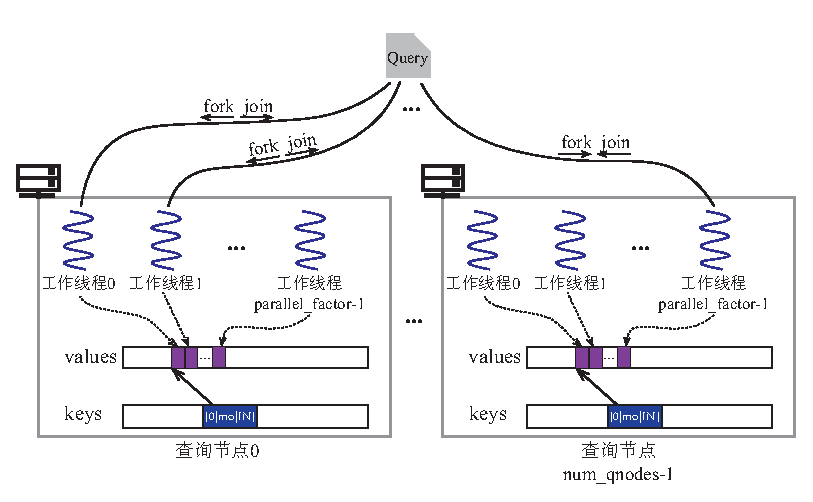
\includegraphics[width=0.75\textwidth]  {figures/fork-join.eps}}
\bicaption{大查询的fork-join过程}{Fork-join process of a heavy query}
\label{fork-join}
\end{figure}

查询引擎在处理小查询时也可能会使用fork-join机制:当工作线程在准备开始执行一个五元模式时,如果中间结果条目数达到系统预设的阈值(例如100),且工作线程需要通过较多跨节点的单边RDMA Read操作来执行该模式,那么工作线程会将其分成\texttt{num\_qnodes}个子查询,然后分别发送给各个查询节点的一个工作线程共同执行。查询的划分实质上是中间结果的划分,中间结果是依据执行该五元模式需要使用的变量的取值划分的,如果某行中间结果中该变量的取值为\texttt{val},那么该行中间结果会被划分到的子查询(从0开始编号)为:
\begin{equation}
    \mathtt{val \ \% \ num\_qnodes}
\end{equation}
查询划分完成后,子查询$i$会被发送到查询节点$i$执行。

只要遵守以上规则,子查询可以被进一步地划分,这样就可能形成一颗以代理线程发来的查询为根节点的查询树。

查询语句执行过程中,一个变量可能处于Unknown和Known两种状态,它们的含义分别为:
\begin{itemize}
    \item Unknown:该变量没有在之前的模式中出现过,当前中间结果表中没有该变量对应的列;
    \item Known:该变量已经在之前的模式中出现过,当前中间结果表中有该变量对应的列。
\end{itemize}

查询引擎在执行时序三元组时间范围模式时,会先从“时序超边存储”中查找所有符合模式指定的时间范围的时序三元组,然后逐一判断每个时序三元组是否与模式的前半部分(即\texttt{interval s p o})匹配。匹配一个时序三元组的方法为:先从\texttt{s}开始,如果它是变量且状态是Unknown,那么该时序三元组的主语就是它的一个可取值;如果它是变量且状态是Known,那么就需要逐一验证中间结果表每一行中该变量对应的列是否与该时序三元组的主语相同,若是则保留该行,否则舍弃该行;如果它是常量,那么只有在该时序三元组的主语与之相同时才可继续匹配。接着以类似过程匹配\texttt{p}、\texttt{o}、\texttt{interval}的\texttt{?var$_1$}和\texttt{?var$_2$}。

查询引擎在执行五元模式时,通常会先从其中的常量开始,通过构造合适的键从分布式键值存储中为模式中的变量寻找可取值,从而将变量的状态从Unknown转移到Known。然后可能会使用中间结果表每一行中Known变量对应的列的值继续构造合适的键进行进一步的图探索,直到所有五元模式都执行完毕。

\section{时序超图存储结构和查询引擎}
时序超图存储的设计思路与时序RDF图存储类似,都使用了分布式键值存储辅以分布式排序数组的存储结构。时序超图查询引擎使用存储层提供的接口逐一执行HQL-T查询语句中的各RP。本节将详细介绍时序超图的存储结构和查询引擎。
\subsection{存储结构}
\label{sec:hyperstore}
系统支持的时序超图数据集格式为\texttt{时序超边类型,时序超边名称,有效时间区间的开始时间,有效时间区间的截止时间,\{顶点名称1,顶点名称2,...\}}。
\sys 同样会将时序超图数据集中的字符串转化成整型ID进行存储。系统默认使用32位UINT表示顶点字符串对应的ID(下称\texttt{vid}),取值范围为$[2^{16}, 2^{32})$,对于顶点数量比较庞大的数据集,可以在系统编译时指定使用64位UINT表示\texttt{vid},取值范围就扩充到$[2^{16}, 2^{48})$。系统使用64位UINT表示时序超边ID(下称\texttt{heid}),取值范围为$[2^{16}, 2^{48})$。值得注意的是,可能有多条时序超边的名称相同,例如字符串“群聊1”可能对应多条时序超边,表示“群聊1”在不同时间区间下的成员情况。系统会给予相同名称的不同时序超边不同的\texttt{heid},在将表示时序超边名称的字符串转换成\texttt{heid}时,字符串服务器返回的是\texttt{heid}的列表。表示时序超边和顶点的类型的字符串对应的ID(下分别称\texttt{htid}和\texttt{tid})的范围为$[2,2^{16})$。

时序超图存储内存布局如图\ref{thyperstore},与时序RDF图存储类似,它分为键值存储区和时序超边存储区两部分。
时序超边存储区存储的是每个超边的ID、类型及其有效时间,即由\texttt{
[超边ID,超边类型,有效时间区间的开始时间,有效时间区间的截止时间]}四元组组成,它本质上也是内存数组。时序超边存储区分为两部分,在“时序超边存储1”中,四元组按照有效时间区间的开始时间升序排布;在“时序超边存储2”中,四元组按照有效时间区间的截止时间升序排布。时序超边的\texttt{heid}与它对应的四元组在“时序超边存储1”中的偏移量\texttt{off}的关系为:
\begin{equation}
    \mathtt{heid = off + 2^{16}}
\end{equation}
键值存储区中的键值对分为直接索引和间接索引两类,在直接索引中,值是实际数据;在间接索引中,值由指向“时序超边存储1”中四元组的指针组成。

\begin{figure}[!htb]
\center{
\includegraphics[width=0.6\textwidth]  {figures/thyperstore.eps}}
\bicaption{时序超图存储内存布局}{Temporal hypergraph storage memory layout}
\label{thyperstore}
\end{figure}

在键值存储区中,各种键值对及其类型如表\ref{tab:thyper}所示,系统使用两个分布式键值存储结构V2E KV和E2V KV来存储这些键值对。
键值对\ding{182}\textasciitilde\ding{184}位于E2V KV,键的数据类型是64位UINT,值的基本数据类型和\texttt{vid}的数据类型相同;键值对\ding{185}\textasciitilde\ding{188}位于V2E KV,键的数据类型也是64位UINT,由高48位和低16位两部分组成,值的基本数据类型是64位UINT。E2V KV中的键值对都是直接索引,V2E KV中的键值对除了\ding{185}外都是间接索引。
\begin{table}[!hpt]
  \bicaption{时序超图存储使用的键值对}{Key-value pairs used in temporal hypergraph storage}
  \label{tab:thyper}
  \centering
  \begin{tabular}{p{1cm}p{2cm}p{8cm}p{3cm}} \toprule
    序号 & 键 & 值 & 类型 \\ \midrule
    \ding{182}\centering & \texttt{[htid]} & 类型为\texttt{htid}的所有时序超边包含的所有\texttt{vid} & \multirow{4}{*}{直接索引} \\
    \ding{183}\centering & \texttt{[tid]} & 类型为\texttt{tid}的所有\texttt{vid} & \\
    \ding{184}\centering & \texttt{[heid]} & 时序超边\texttt{heid}包含的所有\texttt{vid} & \\
    \ding{185}\centering & \texttt{[vid|0]} & 顶点\texttt{vid}的\texttt{tid} & \\ 
    \hline
    \ding{186}\centering & \texttt{[vid|htid]} & 包含顶点\texttt{vid}且类型为\texttt{htid}的所有时序超边 & \multirow{2}{*}{间接索引} \\ 
    \ding{187}\centering & \texttt{[0|htid]} & 类型为\texttt{htid}的所有时序超边 & \\ 
    \bottomrule
  \end{tabular}
\end{table}

图\ref{thsdemo}(a)展示了一个简单的时序超图拓扑,它从微信中的群聊及公众号和微信用户之间的关系抽象而来,它包含两类时序超边:群聊成员和公众号关注者。
有两条类型为群聊成员的时序超边:“群聊1”、“群聊2”,有三条类型为公众号关注者的时序超边:“公众号1”、“公众号2”、“公众号3”,有10个名称分别为A\textasciitilde J的类型为微信用户的顶点。
图\ref{thsdemo}(b)给出了系统会为其生成的一部分键值对。为了便于理解,图中使用字符串表示时序超边、顶点及其类型,系统实际使用的是这些字符串对应的ID。
在间接索引中,值是一个由时序超边对应的四元组在“时序超边存储1”中的偏移量组成的列表,例如,时序超边“群聊2”对应的四元组在“时序超边存储1”中的偏移量为1,那么间接索引就使用1来表示“群聊2”。

\begin{figure}[!htb]
\center{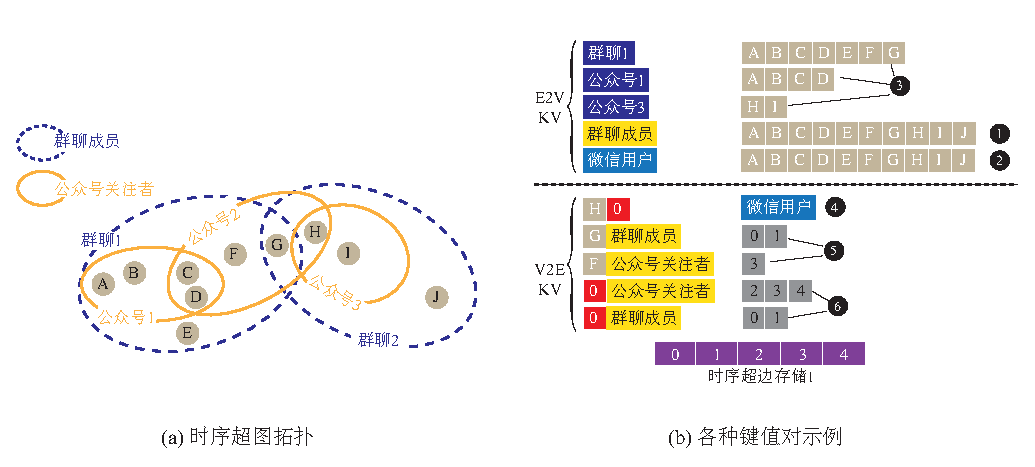
\includegraphics[width=0.95\textwidth]  {figures/thsdemo.eps}}
\bicaption{时序超图存储使用的键值对示例}{Example of key-value pairs used in temporal hypergraph storage}
\label{thsdemo}
\end{figure}

为了实现分布式可扩展存储,系统使用如下规则将键值对和时序超边划分到各查询节点中存储:
\begin{enumerate}
    \item \label{partitionRule1} 每个查询节点负责一块连续ID的时序超边和顶点的管理,时序超边\texttt{heid}会被分配到的查询节点(查询节点从0开始编号)为:
    \begin{equation}
        \mathtt{(heid - 2^{16}) \ / \ \lceil num\_thes \ / \ num\_qnodes \rceil}
    \end{equation}
    其中\texttt{num\_thes}是时序超边总数,\texttt{num\_qnodes}是查询节点数。顶点的分配方法同理。
    \item 对于键值对\ding{182}\ding{183}\ding{187},将值按照\ref{partitionRule1}中的规则划分到各查询节点存储,同一键会出现在每个查询节点的键值存储中;对于键值对\ding{184}\ding{185}\ding{186},将键依据其高48位按照\ref{partitionRule1}中的规则划分到不同查询节点存储,每个键只会出现在一个查询节点的键值存储中。
    \item 将所有四元组分别按有效时间区间的开始时间和截止时间排序后,分别按块划分到各查询节点的“时序超边存储1”和“时序超边存储2”中存储,偏移量为\texttt{off}的四元组会被分配到的查询节点(从0开始编号)为:
    \begin{equation}
        \mathtt{off \ / \ \lceil num\_thes \ / \ num\_qnodes \rceil}
    \end{equation}
\end{enumerate}

\subsection{查询引擎}
HQL-T查询引擎同样沿用了Wukong使用的图探索和全历史剪枝算法。默认情况下,查询引擎会使用存储层提供的接口通过键值存储查找所需的数据,但对于一些以时间点或时间范围为条件的查询,直接在“时序超边存储”上通过二分法查找符合条件的时序超边可能更加高效。例如图\ref{hql}中的查询语句是要查找最后一次成员变动发生于2023年10月1日到2023年10月7日期间的所有群聊及其成员,在执行该语句时,可以使用“时序超边存储1”快速找到有效时间区间开始时间在2023年10月1日到2023年10月7日期间的所有时序超边,然后从中筛选出类型为“群聊成员”且有效时间区间截止时间晚于当前时间的时序超边即可。如果查询引擎不使用“时序超边存储”,而是先从键值存储中找到所有类型为“群聊成员”的时序超边,再筛选出有效时间区间符合条件的时序超边,那么就会带来更大的数据访问开销。目前系统尚未实现HQL-T的查询优化器,无法自动判断使用键值存储和使用“时序超边存储”哪个效率更高。系统的替代方案是将选择权交给用户,由用户在查询语句中使用\textbf{时序超边时间范围模式}显式地指定使用“时序超边存储”进行时间条件查询,语法为:
\begin{equation}
    \mathtt{?var \ STRAT/END(const_1, const_2) \ interval}
\end{equation}

其中变量\texttt{?var}会取值为查询到的时序超边的\texttt{heid};\texttt{START}和\texttt{END}二选一,\texttt{START}指定依据有效时间区间开始时间进行查找,\texttt{END}指定依据有效时间区间截止时间进行查找;\texttt{const$_1$}和\texttt{const$_2$}是两个时间常量且\texttt{const$_1\leq$const$_2$},用于指定要查找的时间范围;\texttt{interval}是可选的,它是一个由两个变量组成的区间,格式为\texttt{[?var$_1$,?var$_2$)},当它存在时,两个变量会分别取值为查询到的时序超边的有效时间区间的开始时间和截止时间。我们规定,时序超边时间范围模式只能出现在GP中最开始的位置,它们会先于RP被处理。值得注意的是,用户需要自行估算使用时序超边时间范围模式是否能够提高查询的执行效率,避免出现负优化。图\ref{guide}中的查询语句与图\ref{hql}中的查询语句含义相同,但它显式地指定使用“时序超边存储1”进行时间范围查询。

\begin{figure}[!htb]
\center{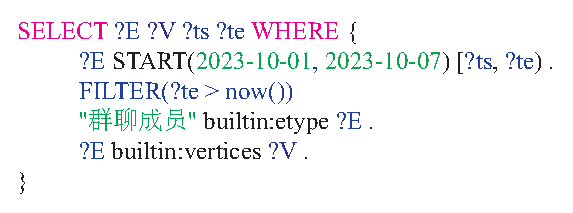
\includegraphics[width=0.55\textwidth]  {figures/guide.eps}}
\bicaption{显式指定使用“时序超边存储”的查询语句示例}{Example of a query that explicitly specifies the use of "temporal hyperedge storage"}
\label{guide}
\end{figure}

与SPARQL-T类似,HQL-T查询语句同样可分为大查询和小查询两类,大查询通常以大量时序超边或顶点作为起始,然后探索更多数量的时序超边和顶点;小查询通常从一个固定的时序超边或顶点开始,访问少量的时序超边和顶点。具体来说,大查询包含以下两类:
\begin{enumerate}
    \item 第一个查询模式是GE或GV模式的查询语句;
    \item 包含时序超边时间范围模式的查询语句。
\end{enumerate}
其他的查询语句都属于小查询。
查询引擎同样使用fork-join机制来处理大查询,其过程与SPARQL-T查询引擎完全相同,在此不作赘述。

查询引擎在处理小查询时同样可能会使用fork-join机制:当工作线程在准备开始执行一个RP时,如果中间结果条目数达到系统预设的阈值(例如100),且工作线程需要通过较多跨节点的单边RDMA Read操作来执行该RP,那么工作线程会将其分成\texttt{num\_qnodes}个子查询,然后分别发送给各个查询节点的一个工作线程共同执行。在划分查询时,中间结果是依据输入元素列表中的第一个变量的取值划分的,如果某行中间结果中该变量的取值为\texttt{val},那么该行中间结果会被划分到的子查询(从0开始编号)为:
\begin{equation}
    \mathtt{(val - 2^{16}) \ / \ \lceil num\_thes \ / \ num\_qnodes \rceil}
\end{equation}

V2E、E2V、V2V和E2E这四种RP的执行比较复杂,执行这些模式时输入元素列表中各变量的状态一定是Known,输出元素列表中变量的状态是Known或Unknown。接下来我们分别详细介绍这四种RP的执行逻辑,我们只讨论输出元素列表中变量的状态是Unknown的情况;对于V2E、E2V和E2E模式,我们只讨论包含\texttt{interval}的情况。
\begin{itemize}
    \item \textbf{V2E模式:}该模式的输入元素列表可以包含若干表示顶点的常量或变量。执行该模式时,首先需要使用键值对\ding{186}分别获取输入元素列表中的各常量对应的\texttt{heid}集合,然后求取这些集合的交集$s_1$。接下来对于每行中间结果,再使用键值对\ding{186}分别获取输入元素列表中各变量取值对应的\texttt{heid}集合,求取这些集合的交集$s_2$,然后求取$s_1$和$s_2$的交集$s$,$s$即是该变量可取值的集合。最后根据\texttt{heid}计算出偏移量,在“时序超边存储1”中读取对应四元组中的生命周期信息即可。
    \item \textbf{E2V模式:}该模式的输入元素列表可以包含若干表示时序超边的常量或变量。输入元素列表中的一个常量可能对应多条时序超边,查询引擎需要首先计算能够使得每个常量对应的时序超边都有且仅有一个有效的所有时间区间,记为$itv_1, itv_2,...,itv_n$(在图\ref{e2v}中是红色虚线标出的三个时间区间),然后对于每一个时间区间,使用键值对\ding{184}分别获取每条有效的时序超边对应的\texttt{vid}集合并求交集,记得到的集合为$s_1, s_2, ..., s_n$。接下来对于每行中间结果,计算能够使得输入元素列表中各变量取值表示的时序超边都有效的最大时间区间,记为$itv$(在图\ref{e2v}中是黑色虚线标出的时间区间,由于每个变量的取值只能表示一条时序超边,所以此处最多计算得到一个时间区间),然后使用键值对\ding{184}分别获取这些时序超边对应的\texttt{vid}集合,求取这些集合的交集$s$,最后将时间区间$itv$分别与时间区间$itv_1, itv_2,...,itv_n$求交,得到新的时间区间$itv_1', itv_2',...,itv_m'$(在图\ref{e2v}中是黑色双向箭头标出的两个时间区间)并计算每个新时间区间上$s_i$和$s$的交集$s_i'$。最终,一行中间结果能够生成$|s_1'|+|s_2'|+...+|s_m'|$行新的中间结果。
    
    \begin{figure}[!htb]
    \center{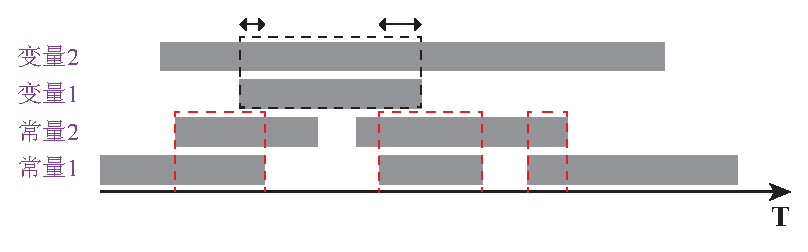
\includegraphics[width=0.6\textwidth]  {figures/e2v.eps}}
    \bicaption{执行E2V模式时对时间区间的处理过程}{Processing of time intervals when executing E2V pattern}
    \label{e2v}
    \end{figure}
    
    \item \textbf{V2V模式:}该模式的输入元素列表可以包含若干表示顶点的常量或变量。执行该模式时,首先要为输出元素列表中的变量寻找候选取值,为此,查询引擎将包含输入元素列表中第一个常量(如果输入元素列表没有常量,则是第一个变量的取值)所表示的顶点的所有时序超边包含的所有顶点作为候选顶点集合。确定候选顶点集合后,查询引擎会逐一验证每个候选顶点是否同时与各输入顶点出现在相同时序超边且时序超边的数量满足参数的要求,验证通过的候选顶点才会作为输出元素列表中变量的取值。
    \item \textbf{E2E模式:}该模式的执行逻辑与E2V模式的执行逻辑相似,此外,执行此模式同样需要为输出元素列表中的变量寻找候选取值,然后验证候选取值是否能够使得参数指定的条件成立。该模式的详细执行过程不再赘述。
\end{itemize}

\section{本章小结}
本章介绍了\sys 时序图查询模块的设计与实现。时序RDF图和时序超图都没有标准的查询语言,所以本文在RDF图查询语言SPARQL的基础上设计了时序RDF图查询语言SPARQL-T,从零开始设计了时序超图查询语言HQL-T。SPARQL-T将SPARQL的GP中的三元模式扩展到五元模式,HQL-T的GP则由基础关系模式(RP)组成。时序RDF图存储和时序超图存储的设计思路类似,都使用了分布式键值存储辅以分布式排序数组的存储结构,键值存储都使用了直接索引和间接索引相结合的设计,在实现了高效的拓扑查询和时间条件查询的同时,减少了时序数据存储占用的空间。
SPARQL-T的时序三元组时间范围模式和HQL-T的时序超边时间范围模式可以用来在特定条件下加速时间条件查询。
SPARQL-T和HQL-T查询引擎都沿用了Wukong使用的图探索和全历史剪枝算法,都使用了fork-join机制来加速复杂查询的执行。
